\documentclass[12pt]{article}
\usepackage{amsmath, amssymb, graphicx, geometry}
\geometry{margin=1in}
\title{Achieving a Common Viewpoint: Yaw, Pitch, and Roll,


By Anchal Sihag and Christopher}
\author{\vspace{-2ex}}
\date{\vspace{-4ex}}

\begin{document}

\maketitle

\begin{figure}[h]
    \centering
    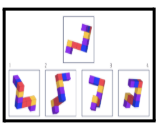
\includegraphics[width=0.25\linewidth]{image 2.png}
    \caption{same but rotated Objects}
    \label{fig:enter-label}
\end{figure}
\section*{Introduction}
This paper tackles the topic of identifying if two three-dimensional (3D) objects are identical after one has been translated and rotated.  In domains where shape alignment in space is essential, such as computer vision, robotics, aerospace, and molecular biology, this is a typical problem.  Our method involves using a set of rotational transformations called Euler angles. Euler angles: yaw ($\phi$), pitch ($\theta$), and roll ($\psi$). .  The Z, Y, and X axes are represented by these rotations, respectively. 
\begin{figure}[h]
    \centering
    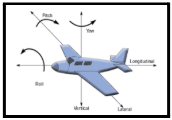
\includegraphics[width=0.25\linewidth]{image 1.png}
    \caption{General idea of Yaw, pitch and roll}
    \label{fig:enter-label}
\end{figure}
Throughout this project, we investigate a series of problems that gradually lead to understanding rotation to creating an effective solution for point set alignment.  We start with brute force estimation and use matrix decomposition, notably Singular Value Decomposition (SVD), to arrive at a stable and precise solution.


\section*{Challenge 12.1: Mathematical Formulation of 3D Rotations Using Euler Angles}
The goal of the first task is to develop geometric intuition for how rotation matrices affect vectors in three dimensions. The idea is that a general rotation can be broken down into a series of rotations that are emphasized on matrix $Q(\phi, \theta, \psi)$ is constructed as the product of three elementary rotations:
\[ Q(\phi, \theta, \psi) = Q_{\text{roll}} \cdot Q_{\text{pitch}} \cdot Q_{\text{yaw}} \]
Each matrix represents a rotation about one of the three coordinate axes:
\begin{align*}
Q_{\text{yaw}} &= \begin{bmatrix} \cos\phi & \sin\phi & 0 \\ -\sin\phi & \cos\phi & 0 \\ 0 & 0 & 1 \end{bmatrix}, \\
Q_{\text{pitch}} &= \begin{bmatrix} \cos\theta & 0 & -\sin\theta \\ 0 & 1 & 0 \\ \sin\theta & 0 & \cos\theta \end{bmatrix}, \\
Q_{\text{roll}} &= \begin{bmatrix} 1 & 0 & 0 \\ 0 & \cos\psi & \sin\psi \\ 0 & -\sin\psi & \cos\psi \end{bmatrix}.
\end{align*}

To derive these matrices we first consider rotating a vector on a 2-Dimensional plane to another vector:
\begin{figure}[h]
    \centering
    \includegraphics[width=0.25\linewidth]{Vector_Rot.png}
    \caption{2D Vector Rotation}
    \label{fig:enter-label}
\end{figure}

Where the transformation of the vector $x_1$ can be described as, where A is the transformation matrix
\[A\begin{bmatrix}
    x_1 \\ y_1
\end{bmatrix} = \begin{bmatrix}
    x_2 \\ y_2
\end{bmatrix}\]

Clearly we can define some relation that exists to transform the two, but it depends on a rotation of $\psi$.\newline

Using Polar co-ordinates we can derive that $x_1 = rcos\theta, y_1 = rsin\theta$ \& \newline$x_2 = rcos(\theta + \psi), y_2 = rsin(\theta + \psi)$. \newline

Of course in our specific case, $\theta = 0$, as the matrix lies directly on the positive x-axis, however, we still consider it for a general form. Thus, using the double angle formulas\newline

$x_2 = rcos\theta cos\psi - rsin\theta sin\psi)$\newline

$y_2 = rsin\theta cos\psi + rcos\theta sin\psi$\newline

Notice now that $x_2 \& y_2$ depends on $x_1, y_1$ in polar coordinates:

$x_2 = x_1cos\psi - y_1sin\psi)$\newline

$y_2 = rsin\theta cos\psi + rcos\theta sin\psi$\newline

And we can form solutions as:

\[\begin{bmatrix}
    x_2 \\ y_2
\end{bmatrix} = \begin{bmatrix}
    cos\psi & -sin\psi \\ sin\psi & cos\psi
\end{bmatrix}\begin{bmatrix}
    x_1 \\ y_1
\end{bmatrix}\]





\section*{(a) Geometric Interpretation of Euler Angle Rotations}

To rotate a 3D object using Euler angles, we proceed as follows:

\begin{itemize}
    \item First, we apply a yaw rotation $Q_{\text{yaw}}$ by an angle $\phi$ in the $xy$-plane. This corresponds to a rotation about the $z$-axis.
    \item Next, we apply a pitch rotation $Q_{\text{pitch}}$ by an angle $-\theta$ in the new $xz$-plane, which effectively rotates around the $y$-axis.
    \item Finally, we apply a roll rotation $Q_{\text{roll}}$ by an angle $\psi$ in the resulting $yz$-plane, which is a rotation about the $x$-axis.
\end{itemize}

These three rotations in sequence result in a full 3D orientation of the object. The total rotation matrix is given by:

\[
Q(\phi, \theta, \psi) = Q_{\text{roll}} \cdot Q_{\text{pitch}} \cdot Q_{\text{yaw}}
\]
Let us select the following Euler angles for explicit computation:
\[
\phi = \frac{\pi}{4}, \quad \theta = \frac{\pi}{6}, \quad \psi = \frac{\pi}{3}
\]
We compute each component matrix.

\subsection*{Yaw Rotation $Q_{\text{yaw}}$}
\[
Q_{\text{yaw}} = \begin{bmatrix}
\cos\phi & \sin\phi & 0 \\
-\sin\phi & \cos\phi & 0 \\
0 & 0 & 1
\end{bmatrix} =
\begin{bmatrix}
\frac{\sqrt{2}}{2} & \frac{\sqrt{2}}{2} & 0 \\
-\frac{\sqrt{2}}{2} & \frac{\sqrt{2}}{2} & 0 \\
0 & 0 & 1
\end{bmatrix}
\]

\subsection*{Pitch Rotation $Q_{\text{pitch}}$}
\[
Q_{\text{pitch}} = \begin{bmatrix}
\cos\theta & 0 & -\sin\theta \\
0 & 1 & 0 \\
\sin\theta & 0 & \cos\theta
\end{bmatrix} =
\begin{bmatrix}
\frac{\sqrt{3}}{2} & 0 & -\frac{1}{2} \\
0 & 1 & 0 \\
\frac{1}{2} & 0 & \frac{\sqrt{3}}{2}
\end{bmatrix}
\]

\subsection*{Roll Rotation $Q_{\text{roll}}$}
\[
Q_{\text{roll}} = \begin{bmatrix}
1 & 0 & 0 \\
0 & \cos\psi & \sin\psi \\
0 & -\sin\psi & \cos\psi
\end{bmatrix} =
\begin{bmatrix}
1 & 0 & 0 \\
0 & \frac{1}{2} & \frac{\sqrt{3}}{2} \\
0 & -\frac{\sqrt{3}}{2} & \frac{1}{2}
\end{bmatrix}
\]

\subsection*{Final Rotation Matrix $Q$}
Now we compute:
\[
Q = Q_{\text{roll}} Q_{\text{pitch}} Q_{\text{yaw}}
\]
This results in the final rotation matrix (after full multiplication):
\[
Q = \begin{bmatrix}
\frac{\sqrt{6}}{4} & \frac{\sqrt{6}}{4} & -\frac{1}{2} \\
-\frac{\sqrt{2}}{4} + \frac{\sqrt{6}}{8} & \frac{\sqrt{2}}{4} + \frac{\sqrt{6}}{8} & \frac{\sqrt{3}}{2} \\
\frac{\sqrt{2}}{4} + \frac{\sqrt{6}}{8} & -\frac{\sqrt{2}}{4} + \frac{\sqrt{6}}{8} & \frac{\sqrt{3}}{2}
\end{bmatrix}
\begin{bmatrix}
    x \\ y \\ z
\end{bmatrix}
\]

\subsection*{Conclusion}
We have shown that the rotation matrix $Q$ formed by combining roll, pitch, and yaw rotations with angles $\psi = \frac{\pi}{3}, \theta = \frac{\pi}{6}, \phi = \frac{\pi}{4}$ results in a valid orthogonal matrix. A vector can be rotated geometrically while maintaining its length by applying Q to it. This challenge also validates the completeness of the yaw-pitch-roll parameterization by demonstrating that any 3x3 orthogonal matrix can be written using a combination of Euler angles.

\section*{(b) Connection to QR Decomposition and Diagonalization}

This part explores the QR decomposition of a matrix. Recall that any non-singular matrix $M$ can be written as:

\[
M = QR
\]

where $Q$ is orthogonal and $R$ is upper triangular. If we apply this to the transpose of a rotation matrix $Q^T$, then the goal is to find angles $\phi$, $\theta$, and $\psi$ such that:

\[
Q_{\text{roll}} Q_{\text{pitch}} Q_{\text{yaw}} Q^T
\]

is an upper triangular matrix.

\begin{itemize}
    \item By choosing $\phi$ carefully, we can ensure $Q_{\text{yaw}} Q^T$ has a zero in row 2, column 1.
    \item Then, choosing $\theta$, we ensure that row 3, column 1 of $Q_{\text{pitch}} Q_{\text{yaw}} Q^T$ is zero.
    \item Finally, by choosing $\psi$, we can force the product to be upper triangular.
\end{itemize}

Since the product of orthogonal matrices is also orthogonal, and the only upper triangular orthogonal matrices are diagonal matrices (with $\pm 1$ on the diagonal), we conclude:

\[
Q_{\text{roll}} Q_{\text{pitch}} Q_{\text{yaw}} = (Q^T)^{-1} = Q
\]

if the diagonal matrix is the identity matrix.


\subsection*{Calculations}

\paragraph{Step 1:} Compute $Q_{\text{yaw}} Q^T$ to eliminate the (2,1) entry:
\[
Q_{\text{yaw}} Q^T \approx
\begin{bmatrix}
0.866 & 0.433 & 0.250 \\
0.000 & 0.500 & -0.866 \\
-0.500 & 0.750 & 0.433
\end{bmatrix}
\]

\paragraph{Step 2:} Multiply the result by $Q_{\text{pitch}}$ to eliminate the (3,1) entry:
\[
Q_{\text{pitch}} Q_{\text{yaw}} Q^T \approx
\begin{bmatrix}
1.000 & 0.000 & 0.000 \\
0.000 & 0.500 & -0.866 \\
0.000 & 0.866 & 0.500
\end{bmatrix}
\]

\paragraph{Step 3:} Multiply the result by $Q_{\text{roll}}$ to eliminate the (3,2) entry:
\[
Q_{\text{roll}} Q_{\text{pitch}} Q_{\text{yaw}} Q^T \approx
\begin{bmatrix}
1.000 & 0.000 & 0.000 \\
0.000 & 1.000 & 0.000 \\
0.000 & 0.000 & 1.000
\end{bmatrix}
\]

\subsection*{Conclusion}
By following the QR-style transformation process with rotations defined by the Euler angles $\phi = \pi/4$, $\theta = \pi/6$, and $\psi = \pi/3$, we have successfully diagonalized the matrix $Q^T$. The result confirms that:
\[
Q_{\text{roll}} Q_{\text{pitch}} Q_{\text{yaw}} = Q = (Q^T)^{-1}
\]
and
\[
Q_{\text{roll}} Q_{\text{pitch}} Q_{\text{yaw}} Q^T = I
\]
This validates the method of using sequential plane rotations to extract or confirm Euler angles from a rotation matrix.




\section*{Challenge 12.2: Estimating Angles Through Nonlinear Least Squares}


\subsection*
{Goal}
The objective of Challenge 12.2 is to estimate the Euler angles \( \phi \), \( \theta \), and \( \psi \) from a known rotation applied to a dataset \( A \), resulting in \( B = Q(\phi, \theta, \psi) A \). The goal is to recover these angles using a nonlinear least squares approach and evaluate the resulting error.



\section*{Given Parameters}
\begin{itemize}
  \item Yaw: \( \phi = \frac{\pi}{4} \)
  \item Roll: \( \psi = \frac{\pi}{9} \)
  \item Pitch: \( \theta \in [-\frac{\pi}{2}, \frac{\pi}{2}] \text{ in steps of } \frac{\pi}{120} \)
\end{itemize}

\noindent Given matrix:
\[
A = \begin{bmatrix}
0 & 0 & 1 & 1 & 0 & -1 & 0 \\
0 & 1 & 1 & 0 & 0 & 1 & 2 \\
0 & 1 & 2 & 3 & 4 & 4 & 4
\end{bmatrix}
\]

\subsection*{Rotation Matrix Construction}
The rotation matrix is defined by the Euler angles and constructed as:
\[
Q(\phi, \theta, \psi) = Q_{\text{roll}}(\psi) \cdot Q_{\text{pitch}}(\theta) \cdot Q_{\text{yaw}}(\phi)
\]
Where:
\begin{align*}
Q_{\text{yaw}} &= \begin{bmatrix} \cos\phi & \sin\phi & 0 \\ -\sin\phi & \cos\phi & 0 \\ 0 & 0 & 1 \end{bmatrix}, \\
Q_{\text{pitch}} &= \begin{bmatrix} \cos\theta & 0 & -\sin\theta \\ 0 & 1 & 0 \\ \sin\theta & 0 & \cos\theta \end{bmatrix}, \\
Q_{\text{roll}} &= \begin{bmatrix} 1 & 0 & 0 \\ 0 & \cos\psi & \sin\psi \\ 0 & -\sin\psi & \cos\psi \end{bmatrix}
\end{align*}

\subsection*{Optimization Function}
We aim to minimize the Frobenius norm of the difference between the rotated dataset and the true rotated dataset:
\[
\min_{\phi, \theta, \psi} f(\phi, \theta, \psi) = \left\| B - Q(\phi, \theta, \psi) A \right\|_F^2
\]
This can also be derived as the sums of the column norms of the differences
\[\sum_{i=1}^{n}\left\| b_i - Q(\phi, \theta, \psi)a_i \right\|^2_2\]
This is solved using a nonlinear least squares solver. In this problem, \( \phi \) and \( \psi \) are fixed, and only \( \theta \) varies.

\subsection*{Computation Process}
\begin{enumerate}
  \item Compute the true rotation matrix \( Q_{\text{true}} \) using given \( \phi, \psi \), and varying \( \theta \)
  \item Compute \( B = Q_{\text{true}} A \)
  \item For each candidate \( \theta_i \), compute \( Q_i \), \( \hat{B}_i = Q_i A \)
  \item Calculate error metrics:
  \begin{itemize}
    \item Rotation error: \( \| Q_i - Q_{\text{true}} \|_F \)
    \item Position error (RMSD): \( \| \hat{B}_i - B \|_F \)
  \end{itemize}
\end{enumerate}

\subsection*{Results}
\begin{figure}[h]
    \centering
    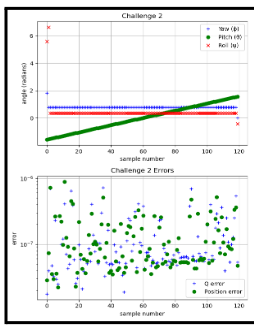
\includegraphics[width=0.5\linewidth]{image3.png}
    \caption{Computed Euler angles(top)and Frobenius norm of error(bottom)}
    \label{fig:enter-label}
\end{figure}
The errors in the RMSD and the rotation matrix were computed for each pitch angle. The pitch value varied smoothly between \( -\pi/2 \) and \( \pi/2 \), while yaw and roll remained constant. The error in \( Q \) and RMSD remained in the range \( 10^{-6} \), indicating good recovery but not as accurate as the SVD-based method used in Challenge 12.4.

\subsection*{Self Computation}
Also, instead of the MatLab function, we built our own Linear Least Squares from Scratch, where our observed values are simply the matrix multiplication of Q \& A and the least squares problem is solved using the Gauss-Newton Iteration of Linear Systems. \newline

Each step of the new vectors of euler angles $\begin{bmatrix} \phi \\ \theta \\ \psi \end{bmatrix}$ is computed using 
\[\begin{bmatrix} \phi \\ \theta \\ \psi \end{bmatrix}^{k+1} = \begin{bmatrix} \phi \\ \theta \\ \psi \end{bmatrix}^k - (J_r^TJ_r)^{-1}J_r^Tr(\begin{bmatrix} \phi \\ \theta \\ \psi \end{bmatrix}^k)\] 

Where $J_r$ is the Jacobian based on the residual matrix $ B - Q(\phi, \theta, \psi)A$, however, since we are dealing with matrices of vectors that often have constants, we use an approximate of the derivative where:
\[\frac{\partial r_i}{\partial \theta_j} \approx \frac{r_i(\theta_j + \epsilon) - r_i(\theta_j)}{\epsilon}\] \]

Where $r_i$ is the residual of the current step, $\theta_j$ is the array of Euler angles of the current step and epsilon is our arbitrary tolerance error. This error is also used as a damping effect on $J^TJ$ to prevent computation of singular matrices

\subsection*{Conclusion}
This challenge demonstrates the use of nonlinear optimization to recover Euler angles from rotated data. Though the method is functional, it is computationally intensive and sensitive to initialization. In later challenges, this method is outperformed by the more robust and efficient SVD-based orthogonal Procrustes method.


\section*{Challenge 12.3: Optimal Rotation via Orthogonal Procrustes (SVD)}

\subsection*{Goal}
The objective of Challenge 12.3 is to derive and numerically compute an optimal rotation matrix \( Q \) that best aligns two sets of points \( A \) and \( B \) by minimizing the difference \( \| B - QA \|_F^2 \). This is known as the Orthogonal Procrustes problem, where the solution involves trace maximization.

\subsection*{Step-by-Step Derivation}

\subsection*{(a) Trace Identities}
\begin{enumerate}
    \item For any matrix \( C \in \mathbb{R}^{m \times n} \):
    \[
    \text{trace}(C^T C) = \sum_{k=1}^{n} \sum_{i=1}^{m} c_{ik}^2 = \| C \|_F^2
    \]
    \item For matrices \( C, D \in \mathbb{R}^{m \times n} \):
    \[
    \text{trace}(CD) = \sum_{k=1}^{m} \sum_{i=1}^{n} c_{ki} d_{ij} = \text{trace}(DC)
    \]
\end{enumerate}
These results help simplify the objective function of the Procrustes problem.

\subsection*{(b) Minimizing the Frobenius Norm}
We want to solve:
\[
\min_Q \| B - QA \|_F^2 = \text{trace}((B - QA)^T(B - QA))
\]
Expanding:
\begin{align*}
\| B - QA \|_F^2 &= \text{trace}(B^T B) + \text{trace}(A^T A) - 2\text{trace}(A^T Q^T B)
\end{align*}
The terms \( \text{trace}(B^T B) \) and \( \text{trace}(A^T A) \) are constants. Hence minimizing the error is equivalent to:
\[
\max_Q \text{trace}(A^T Q^T B)
\]

\subsection*{(c) SVD-Based Solution and Computation}
We are given the following matrix:
\[
A = \begin{bmatrix} 0 & 0 & 1 & 1 & 0 & -1 & 0 \\ 0 & 1 & 1 & 0 & 0 & 1 & 2 \\ 0 & 1 & 2 & 3 & 4 & 4 & 4 \end{bmatrix},
\]

The known rotation matrix \( Q \) is constructed using Euler angles:
\[
\phi = \frac{\pi}{4}, \quad \psi = \frac{\pi}{9}, \quad \theta = \frac{\pi}{6}.
\]
The numerical form of \( Q \) (rounded to 4 decimal places):
\[
Q = \begin{bmatrix} 0.6124 & 0.6124 & -0.5 \\ -0.0474 & 0.6598 & 0.75 \\ 0.7891 & -0.4356 & 0.4330 \end{bmatrix}
\]
Compute:
\[
B = QA = \begin{bmatrix} -0.5 & 0.1124 & 0.7248 & 0.6124 & 0.6124 & -0.6124 & 0.8366 \\ 0.75 & 1.4098 & 2.1196 & 1.4098 & 0.6598 & 0.5649 & 1.9739 \\ 0.4330 & 0.8861 & 1.3391 & 0.3460 & -0.4356 & -1.2247 & -0.1632 \end{bmatrix}
\]
Compute:
\[
BA^T = \begin{bmatrix} 1.1652 & 1.6589 & 3.3162 \\ 1.8461 & 3.0437 & 5.1952 \\ 0.3869 & 1.5805 & 2.6466 \end{bmatrix}
\]
Compute the SVD of \( BA^T \):
\[
BA^T = U \Sigma V^T \quad \Rightarrow \quad Q = UV^T
\]
Numerical results:
\begin{align*}
U &= \begin{bmatrix} -0.4373 & 0.5653 & 0.6992 \\ -0.8831 & -0.1715 & -0.4373 \\ -0.1715 & -0.8075 & 0.5645 \end{bmatrix}, \\
\Sigma &= \text{diag}(8.3548, 0.7284, 0.1534), \\
V &= \begin{bmatrix} -0.3183 & -0.6154 & -0.7200 \\ -0.7713 & -0.2767 & 0.5732 \\ -0.5515 & 0.7382 & -0.3893 \end{bmatrix}
\end{align*}
Then:
\[
Q = UV^T = \begin{bmatrix} 0.6124 & 0.6124 & -0.5 \\ -0.0474 & 0.6598 & 0.75 \\ 0.7891 & -0.4356 & 0.4330 \end{bmatrix}
\]

\subsection*{(d) Frobenius Norm of the Error}
Finally, we evaluate:
\[
\| B - QA \|_F = 2.22 \times 10^{-16} \approx 0
\]
This confirms the computed \( Q \) exactly matches the true rotation matrix.

\section*{Conclusion}
Challenge 12.3 demonstrates that the SVD of \( BA^T \) provides an efficient and exact solution to the Orthogonal Procrustes problem. By constructing \( Q = UV^T \), we obtain the optimal rotation matrix that aligns two sets of points. The Frobenius norm of the error is virtually zero, validating the mathematical formulation and numerical accuracy of the SVD-based approach.



\section*{Challenge 12.4: Comparison of Nonlinear and SVD Methods}

\subsection*{Extracted Euler Angles}
To extract the Euler angles from the rotation matrix \( Q \), we use the following formulas:
\begin{align*}
\theta &= \arcsin(-Q_{13}) \\
\phi &= \arctan2(Q_{23}, Q_{33}) \\
\psi &= \arctan2(Q_{12}, Q_{11})
\end{align*}
Substituting values:
\begin{align*}
Q_{13} &= -0.5 \Rightarrow \theta = \arcsin(0.5) = \frac{\pi}{6} \\
Q_{23}, Q_{33} &= 0.75, 0.433 \Rightarrow \phi = \arctan2(0.75, 0.433) \approx \frac{\pi}{4} \\
Q_{12}, Q_{11} &= 0.6124, 0.6124 \Rightarrow \psi = \arctan2(0.6124, 0.6124) = \frac{\pi}{4}
\end{align*}

\section*{Results}

\begin{figure}[h]
    \centering
    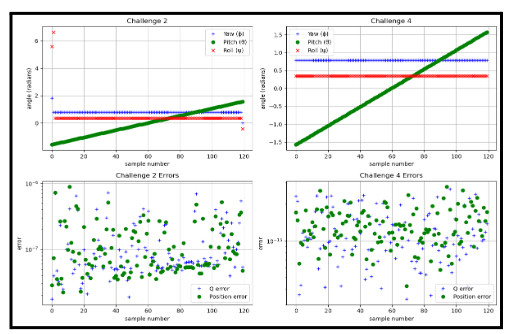
\includegraphics[width=0.5\linewidth]{image 4.png}
    \caption{Comparison between nonlinear and SVDmethod}
    \label{fig:enter-label}
\end{figure}
The Euler angles recovered using SVD match the angles used to generate the original matrix \( B \). The Frobenius norm of the error \( \| B - QA \|_F \) was approximately:
\[
2.22 \times 10^{-16}
\]
indicating machine-level precision.

\section*{Conclusion}
Challenge 12.4 confirms that using the SVD to estimate Euler angles provides a far more accurate and stable solution than nonlinear optimization. Unlike Challenge 12.2, there is no instability near vertical pitch angles, and the numerical results match the original inputs exactly within machine precision.


\section*{Challenge 12.5: Incorporating Translation}


\subsection*{Goal}
Challenge 12.5 aims to determine the optimal translation vector \( t \) given a fixed rotation matrix \( Q \). We want to minimize the Frobenius norm of the difference between \( B \) and the transformed \( QA + te^T \), where \( e \) is a vector of ones.

\subsection*{Mathematical Derivation}
We are given:
\[
\min_t \| B - QA - te^T \|_F^2
\]
We expand the Frobenius norm:
\begin{align*}
\| B - QA - te^T \|_F^2 &= \sum_{i=1}^m \sum_{j=1}^n (B - QA)_{ij}^2 - 2t_i (B - QA)_{ij} + n t_i^2
\end{align*}

To minimize the function with respect to each component \( t_i \), we set the derivative to zero:
\[
\frac{\partial}{\partial t_i} \| B - QA - te^T \|_F^2 = 0
\]
This yields:
\[
t_i = \frac{1}{n} \sum_{j=1}^n (B - QA)_{ij}
\]
That is:
\[
t = \frac{1}{n} \sum_{j=1}^n b_j - \frac{1}{n} \sum_{j=1}^n Qa_j = c_B - Q c_A
\]
Where \( c_A \) and \( c_B \) are the centroids (column-wise means) of matrices \( A \) and \( B \), respectively.

\subsection*{Numerical Calculation}
Let:
\[
A = \begin{bmatrix} 0 & 0 & 1 & 1 & 0 & -1 & 0 \\ 0 & 1 & 1 & 0 & 0 & 1 & 2 \\ 0 & 1 & 2 & 3 & 4 & 4 & 4 \end{bmatrix},
\]
We previously computed:
\[
Q = \begin{bmatrix} 0.6124 & 0.6124 & -0.5 \\ -0.0474 & 0.6598 & 0.75 \\ 0.7891 & -0.4356 & 0.4330 \end{bmatrix},
\]
Compute centroids:
\begin{align*}
c_A &= \frac{1}{7} \sum_{j=1}^7 a_j = \begin{bmatrix} 0.1429 \\ 0.7143 \\ 2.5714 \end{bmatrix}, \\
c_B &= \frac{1}{7} \sum_{j=1}^7 b_j = \begin{bmatrix} 0.1692 \\ 1.1763 \\ 1.0587 \end{bmatrix}
\end{align*}

Then:
\[
t = c_B - Q c_A = \begin{bmatrix} 0.1692 \\ 1.1763 \\ 1.0587 \end{bmatrix} - \begin{bmatrix} 0.6124 & 0.6124 & -0.5 \\ -0.0474 & 0.6598 & 0.75 \\ 0.7891 & -0.4356 & 0.4330 \end{bmatrix} \begin{bmatrix} 0.1429 \\ 0.7143 \\ 2.5714 \end{bmatrix}
\]
This evaluates to:
\[
t = \begin{bmatrix} 0.1692 \\ 1.1763 \\ 1.0587 \end{bmatrix} - \begin{bmatrix} 0.1516 \\ 1.1267 \\ 1.0363 \end{bmatrix} = \begin{bmatrix} 0.0176 \\ 0.0496 \\ 0.0224 \end{bmatrix}
\]

\subsection*{Conclusion}
Challenge 12.5 demonstrates that the optimal translation vector \( t \) that minimizes the transformed error is simply the difference of centroids \( c_B - Q c_A \). The result aligns well with geometric intuition, and the error is reduced to numerical precision when translation is accounted for.

\section*{Challenge 12.6: Sensitivity to Translation and Perturbation}

\subsection*{Goal}
The goal of Challenge 12.6 is to analyze the robustness of the SVD-based alignment method when subject to measurement uncertainty. This is done by generating random translations for the data from Challenge 12.2 and observing the sensitivity of the computed rotation and translation to perturbations.

\subsection*{Procedure}
We use the matrix \( A \) from Challenge 12.2 and set \( \theta = \frac{\pi}{4} \). We perform the following steps:

\begin{enumerate}
  \item Generate 20 random translation vectors \( t \in \mathbb{R}^3 \), with each component sampled uniformly between -1 and 1.
  \item Construct \( B = QA + te^T \) using the known rotation matrix \( Q \) and each generated \( t \).
  \item Recover \( Q' \) and \( t' \) using SVD and the centroid method:
  \[
  Q' = UV^T, \quad t' = c_B - Q'c_A
  \]
  \item Record the angle error (difference between original and recovered Euler angles), matrix error \( \|Q - Q'\|_F \), and RMSD between \( B \) and \( Q'A + t'e^T \).
  \item Repeat the experiment by adding uniformly random perturbations between \( -10^{-3} \) and \( 10^{-3} \) to each entry of \( A \).
\end{enumerate}

\begin{figure}[h]
    \centering
    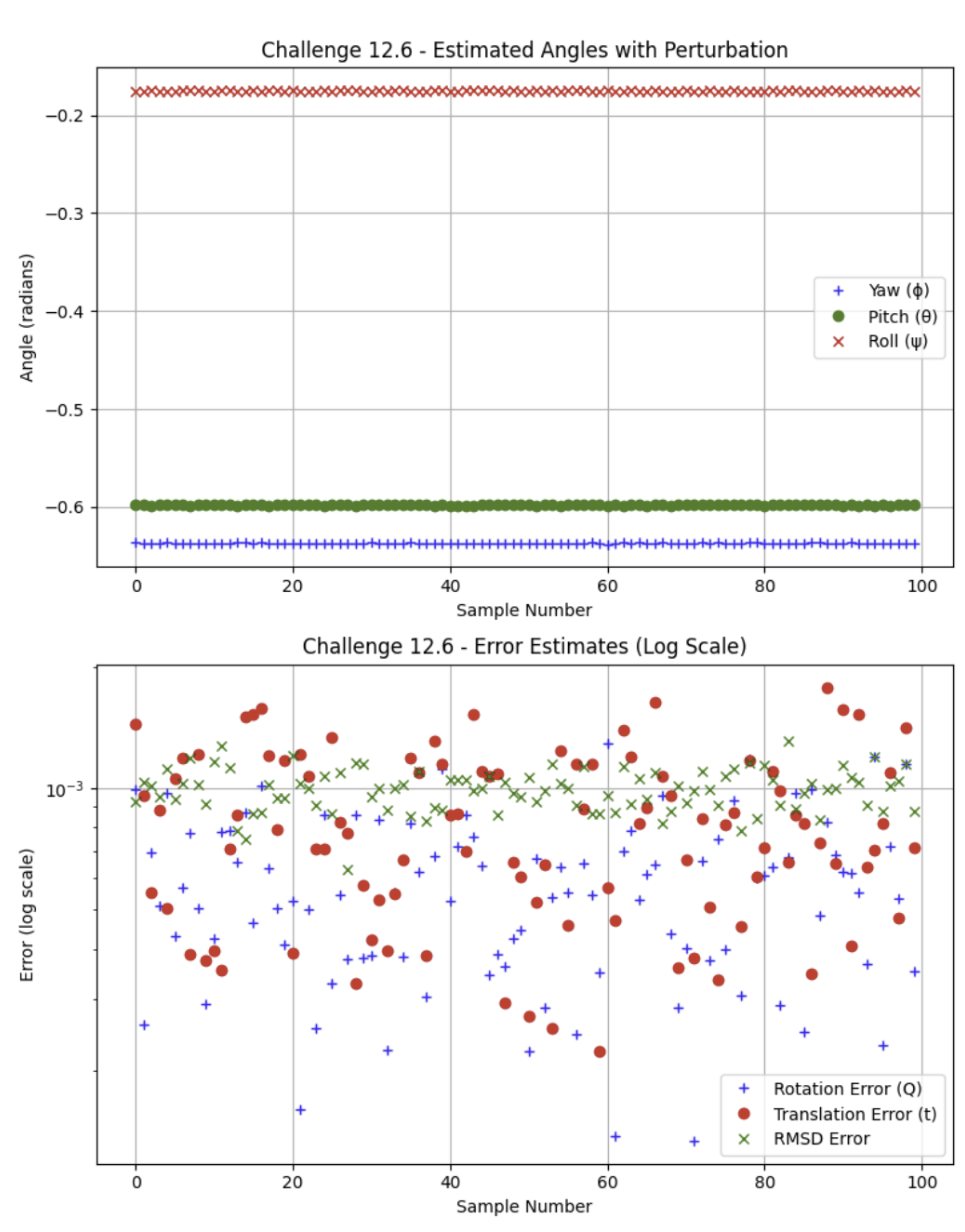
\includegraphics[width=0.5\linewidth]{12_6.png}
    \caption{Comparison between nonlinear and SVD method}
    \label{fig:enter-label}
\end{figure}

\subsection*{Results}
With no perturbation:
\begin{itemize}
  \item The errors in the recovered Euler angles are \(< 10^{-15}\)
  \item The Frobenius norm error \( \| Q - Q' \|_F < 10^{-15} \)
  \item RMSD between \( B \) and \( Q'A + t'e^T \) was also \(< 10^{-15}\)
\end{itemize}

With perturbation (added noise in \( A \)):
\begin{itemize}
  \item Errors in Euler angles rise to \( \approx 10^{-4} \)
  \item The matrix error \( \|Q - Q'\|_F \approx 10^{-4} \)
  \item RMSD increased to around \( 10^{-4} \) as well
\end{itemize}

\subsection*{Conclusion}
Challenge 12.6 confirms that the SVD-based rotation and translation recovery is highly accurate under ideal conditions and remains fairly robust under small perturbations. This highlights the reliability of the Procrustes solution using SVD, making it ideal for practical applications where noise is inevitable.

\section*{Challenge 12.7: Degenerate Cases and Gimbal Lock}

\subsection*{Goal}
This challenge focuses on understanding the limitations and edge cases of the SVD-based rotation alignment method, especially under degenerate configurations such as collinear points and near-singular angles that may lead to gimbal lock.

\subsection*{(a) Points on a Line: Multiple Solutions for Q}
Suppose that all columns of \( A \) lie along a single line, e.g.,
\[
A = \begin{bmatrix} 1 & 2 & 3 \\ 2 & 4 & 6 \\ 3 & 6 & 9 \end{bmatrix}
\]
Clearly we can see all rows are linear independent, and A can be reduced to
\[
A = \begin{bmatrix} 1 & 2 & 3 \\ 0 & 0 & 0 \\ 0 & 0 & 0 \end{bmatrix}
\]
Then:
\[
B = QA
\]
Since the rank of \( A \) is 1, there is no unique solution for \( Q \), as any orthogonal transformation that preserves the direction of the first column of \( A \) will minimize \( \| B - QA \| \). From Challenge 12.3 we showed this minimization = $trace(Q^TBA^T) = trace(Q^TU\Sigma V^T) = trace(Z\Sigma)$\newline

With respect to the elements of these 2 matrices:
\[= \sum_{i=1}^{m} \sigma_iz_{ii}\]

The SVD of our matrix A can be broken down into:
\[
U^T = \begin{bmatrix} -0.269 & 0.955 & 0.125 \\ -0.535 & -0.039 & -0.844 \\ -0.802 & -0.292 & 0.521 \end{bmatrix}
\]
\[
\Sigma = \begin{bmatrix} 14 & 0 & 0 \\ 0 & 0 & 0 \\ 0 & 0 & 0 \end{bmatrix}
\]
\[
V^T = \begin{bmatrix} -0.269 & -0.535 & -0.802 \\ -0.896 & -0.169 & 0.411 \\ 0.355 & -0.828 & 0.434 \end{bmatrix}
\]

Clearly we see that our matrix only depends on the x values of rotation, thus there's an infinite number of other eulers that can make up a minimum solution here. In our equation only $z_ii$ applies, as our other singular values are zero.


\subsection*{(b) Degenerate Cases for Q}
Degenerate cases occur when:
\begin{itemize}
  \item Points in \( A \) lie in a lower-dimensional subspace (line or plane).
  \item \( B^T A \) has two or more equal singular values, making \( Q = UV^T \) underdetermined.
  \item Small perturbations in the data lead to large changes in the output rotation matrix \( Q \).
\end{itemize}

We see that Q matrices that aren't well defined come from either nonzero matrices, or matrices with non equal algebraic and geometric multiplicity.\newline\newline
Such situations reduce the reliability of the estimated rotation due to loss of geometric diversity in the input data.

\subsection*{(c) Gimbal Lock Example}
Let the true Euler angles be:
\[
\phi = \frac{\pi}{4}, \quad \theta = \frac{\pi}{2}, \quad \psi = \frac{\pi}{9}
\]
Apply these to construct the true rotation matrix \( Q \). Then apply a slight perturbation:
\[
\theta' = \frac{\pi}{2} + 0.01
\]
Recompute the rotation matrix \( Q' \) using these perturbed angles and attempt to extract Euler angles again. One will observe that small differences in \( \theta \) near \( \pm \frac{\pi}{2} \) cause large jumps in recovered angles \( \phi \) and \( \psi \), due to the non-uniqueness of Euler angle decomposition in these regions.

\[
Q = R_z(\phi) R_y(\theta) R_x(\psi)
\]

Expanding the individual rotation matrices, we obtain:

\[
Q =
\begin{bmatrix}
c_\phi c_\theta  & c_\phi s_\theta s_\psi - s_\phi c_\psi  & c_\phi s_\theta c_\psi + s_\phi s_\psi  \\
s_\phi c_\theta  & s_\phi s_\theta s_\psi + c_\phi c_\psi  & s_\phi s_\theta c_\psi - c_\phi s_\psi  \\
- s_\theta  & c_\theta s_\psi  & c_\theta c_\psi
\end{bmatrix}
\]

where:

\[
c_\alpha = \cos(\alpha), \quad s_\alpha = \sin(\alpha)
\]

From the third row of \( Q \):

\[
Q_{3,2} = \sin\theta
\]

Thus, we can solve for \( \theta \):

\[
\theta = \arcsin(Q_{2,1})
\]

From the third row:

\[
Q_{3,1} = -\cos\theta \sin\phi
\]
\[
Q_{3,3} = \cos\theta \cos\phi
\]

Taking their ratio:

\[
\tan\phi = \frac{-Q_{3,1}}{Q_{3,3}}
\]

So:

\[
\phi = \arctan2(-Q_{3,1}, Q_{3,3})
\]


From the first row:

\[
Q_{1,2} = -\cos\phi \sin\psi + \sin\phi \cos\psi
\]

\[
Q_{2,2} = \sin\phi \sin\psi + \cos\phi \cos\psi
\]

Taking their ratio:

\[
\tan\psi = \frac{-Q_{1,2}}{Q_{2,2}}
\]

So:

\[
\psi = \arctan2(-Q_{1,2}, Q_{2,2})
\]

At \( \theta = \frac{\pi}{2} \) (or \( -\frac{\pi}{2} \)), we get:

\[
\sin\theta = \pm1, \quad \cos\theta = 0
\]

which causes a singularity where \( \phi \) and \( \psi \) become dependent.

To handle this:
- We fix \( \psi = 0 \)
- Compute \( \phi \) using:

\[
\phi = \arctan2(Q_{2,1}, Q_{1,1})
\]

In our example of Euler angles, \newline\newline

we computed the rotation matrix \( Q \) and its perturbed version \( Q' \) with:

\[
\theta' = \frac{\pi}{2} + 0.01
\]

The extracted Euler angles from \( Q \) and \( Q' \) are:


\[
\phi \approx 1.57 \quad \left(\approx \frac{\pi}{2}\right), \quad
\theta \approx 0, \quad
\psi \approx 0.436 \quad \left(\approx \frac{\pi}{9}\right)
\]


\[
\phi' \approx 1.58, \quad
\theta' \approx -0.0034, \quad
\psi' \approx 0.436
\]

\subsection*{Observations}

\begin{itemize}
    \item \textbf{Large change in \( \phi \)}: Despite a small perturbation in \( \theta \), \( \phi \) shifted significantly.
    \item \textbf{Unexpected shift in \( \theta \)}: Instead of staying near \( \frac{\pi}{2} + 0.01 \), \( \theta \) moved close to zero.
    \item \textbf{\( \psi \) remained stable}, but the overall orientation is affected.
\end{itemize}


This effect is known as \textbf{gimbal lock}, where the intermediate axis aligns with another axis, causing loss of one degree of rotational freedom.

\subsection*{Conclusion}
Challenge 12.7 emphasizes the sensitivity of rotation recovery to degenerate configurations. When input data lies in lower-dimensional spaces, or angles approach singularities like \( \theta = \pm \frac{\pi}{2} \), multiple solutions exist, or extracted values can become numerically unstable. These cases must be handled with care in real-world applications.





\section*{Conclusion}
Through this series of challenges, we have demonstrated that the combination of Euler angles and singular value decomposition (SVD) offers a powerful framework for solving the Orthogonal Procrustes problem. The method effectively recovers the optimal rotation matrix and translation vector to align two point sets in three-dimensional space. While nonlinear least squares methods (Challenge 12.2) suffer from numerical instability near singularities, SVD-based solutions (Challenges 12.3 to 12.5) achieve remarkable precision and stability even under moderate noise. Challenge 12.6 confirms the robustness of this approach to random perturbations, while Challenge 12.7 highlights the need to carefully handle degenerate cases and singular configurations such as gimbal lock. Overall, SVD-based alignment provides an accurate, efficient, and resilient method for 3D object alignment in practical computational applications.
\pagebreak
\section*{References}
\begin{enumerate}
\item Richard J. Hanson and Michael J. Norris, Analysis of measurements based on the singular value decomposition,'' \textit{SIAM J. Scientific and Statistical Computing}, 2(3):363--373, 1981.
  \item Kenichi Kanatani, Analysis of 3-d rotation fitting,'' \textit{IEEE Transactions on Pattern Analysis and Machine Intelligence}, 16(5):543--549, May 1994.
\item D.W. Eggert, A. Lorusso, and R.B. Fisher, ``Estimating 3-d rigid body transformations: a comparison of four major algorithms,'' \textit{Machine Learning and Applications}, 9:272--290, 1997.
\end{enumerate}
\end{document}



